\chapter{Related research}

% You will need to describe what has been done before and you will need to discuss the theory that your work is based upon. This is a slightly dangerous: Take care not to punish the reader with hairy theory without explaining why it is needed.

% What is the main idea? What is the contribution (the new or interesting thing)? What is important for you? Where it is presented?

% Gist + My comment
% TODO: go through each paper and make short notes on what's important and why.


% ---------------------------------------------------------------------
\section{Wrapper induction method overview}
% discuss classification and state our focus

The problem of data extraction (from web pages?) has been addressed in a number of papers. \cite{Laender:2002:BSW:565117.565137} reviews multiple techniques for generating wrappers, inluding natural language processing, languages and grammar, machine learning, information retrieval, databases, and ontologies. A common goal of all wrapper generation tools is to build a wrapper that is both accurate and robust, but is built with the least possible human interaction. The article provides a taxonomy for grouping wrapping techniques.

The most relevant category mentioned in the paper is the HTML-aware tools. These rely on structural features of HTML documents. The document is parsed into a tree structure and extraction rules are applied to the tree. Altough the tools discused (XWRAP, W4F, RoadRunner) provide a high degree of automation, many of them rely on heuristics and have a weak notion of robustness.

In a more recent overview of web data extraction techniques \cite{Chang:2006:SWI:1159162.1159300} the author argues, that due to template generated content, web IE problems can take advantage machine learning and pattern matching methods. Compare it to traditional IE approaches that are mostly based on natural language processing (NLP). Unsupervised approaches can only support template pages. The extension of such systems to non-template page extraction tasks is very limited.

As our research focus is data extraction from HTML documents which are semi-structured, we focus on techniques based on structural features rather than vague NLPs that require large training sets. Yet the content models are interesting direction for extra accuracy.


% ---------------------------------------------------------------------
\section{HTML aware data extraction}
% elaborate on the research in the area of our focus

% IBM Report: Robust Web Data Extraction with XML Path Expressions
One the the first papers to discuss XPath based wrappers was \cite{Myllymaki02robustweb}. In this approach, XML tools are used convert HTML document into pure XHTML and XPath queries extract desired pieces of information. The wrapper is a set of XSLT extraction rules, i.e. hops that are based on structure, attributes, or content. Yet the actual XPath queries were written by hand without any automation.

The same paper mentions robustness as a feature of a good extraction rule. The author informally defines robustnes as the ability to extract intended data from an HTML page after structural changes to the page. Two metrics for measuring robustness are introduced. The first is a number of times that expression failed to extract correct results. The second is expression complexity in terms of depth. The paper defines a notion of anchors (DOM tree nodes) and hops (relative XPath expressions) over a normalized HTML document. 

% Relative vs absolute queries: Robust Web Contet Extraction
Some techniques \cite{Chang:2006:SWI:1159162.1159300} improve the robustness of XPath expression. The general approach of these techniques is to rewrite the expression into a more robust relative one by tracking structural changes in the traning set. \cite{Kowalkiewicz:2006:RWC:1135777.1135928} empirically confirmed that there is a notable difference between various versions of wrappers in terms of robustness – relative XPath expressions outperform absolute ones significantly. This proves the idea that some wrappers are more robust.

% Vertex tool
\cite{DBLP:conf/icde/GulhaneMMRRSSTT11} introduces apriori style algorithm for learning xpath-based extraction rules that are robust to variations in site structure. Algorithm learns rules from human annotated pages based on structural features. Based on domain knowledge, these features are classified into strong (e.g. HTML attributes \texttt{class} or \texttt{id}, tags, textual fragments) and weak (e.g. \texttt{font}, \texttt{width} attributes). This method tries to build a path from strong features only by generating and combining candidates. If Apriori fails to output precise XPath, Naive-Bayes based classifier is used to evaluate the best guess of newly generated nodes with weak features. Essentially this method is based on enumeration, which makes it slow for large websites. Additional limitations are the use of large training set and that it requires a set of annotated pages for certain heuristics (e.g. support metrics) to properly work. 

% WebSelF tool
\cite{Thomsen:2012:WWS:2364120.2364156} presents a framework that takes into account not only the structure and the content of a scrapped page, but also the context and the presentation, i.e. the location where the data is physically located after full rendering and applying stylesheets. It also works with dynamic page elements, that are frequent in JavaScript rich web pages. The design of the framework consists of three type of functions: for selecting elements, for for verifying the selected elements, and for maintaining the previous functions.

- http://www.cs.uic.edu/~liub/WebMiningBook.html\\


% ---------------------------------------------------------------------
\section{Tree-Edit Models}

% Zhang-Shasha edit-tree distance
To compare similarity of two HTML documents we can use string edit distance or tree edit distance, because of DOM tree. A distance between two ordered trees is considred to be the weighted number of edit operations (insert, edit, delete) to transform on tree into another \cite{shasha1990a}.

% Automatic web news extraction using tree edit distance by Reis'04
In \cite{de2004a} author introduces \emph{Restricted Top-Down Mapping} algorithm, which calculates edit-tree distance by efficiently analysing tree structure. Generally, the algorithm imposes top-down mappings which allow removal and inserts at the bottom of the tree only. Informally, we expect some minor changes inside templates, i.e. just the content at the bottom of the elements.

% Broom analogy
The paper \cite{de2004a} instroduces the idea of tree extractor, i.e. tree structure with wildcards for matching HTML documents. This step recognizes common pattern between two trees. Basically, the template is reconstructed from multiple HTML fragments.

% TODO
- A Survey on Tree Edit Distance and Related Problems\\

% TODO
- RTED - A Robust Algorithm for the Tree Edit Distance\\

% TODO
- Simple fast algorithms for the editing distance between trees and related problems\\

% TODO
- React’s diff algorithm\\

Probabilistic model allow to formalize robustness.

% Robust Web Extraction - An Approach Based on a Probabilistic Tree-Edit Model\\
Dalvi et al. views page evolution as a stochastic process, where individual edit operations (delete, insert and substitution) are picked by their probability \cite{dalvi2009a}. Introduces algorithm for efficiently estimating the probability of one tree evolving into the other. In other words, provides a first formal definition of robustness. Generates a set of candidate XPath wrappers and selects the most robust one.

% Edit cost / Change model
In \cite{de2004a} two tree similarity threshold as fixed constant of 80\%. Every vertex insertion, removal or replacement has unit cost of one. In \cite{dalvi2009a} the probability distribution of the next page state is based on structural patterns in the training set.

% Robust web extraction framework
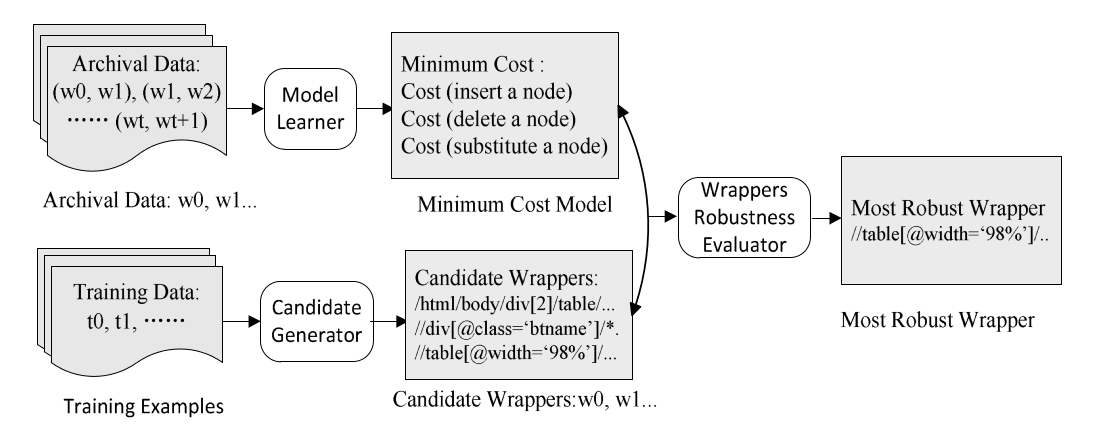
\includegraphics[width=\linewidth]{figures/robust-web-extraction-framework}


- Optimal Schemes for Robust Web Extraction\\
- Robust Web Content Extraction\\
- Robust Web Extraction Based on Minimum Cost Script Edit Model\\
- Robust Web Data Extraction - A Novel Approach Based on Minimum Cost Script Edit Model\\


% ---------------------------------------------------------------------
\section{Data record mining}

\paragraph{Mining Data Records in Web Pages.} Template recognition by string matching. Each node is compared to siblings, if they are generated from same template. If so, form a region.

\paragraph{Efficient recorrd-level wrapper induction.} Broom for record-level wrapping. Extracts templates from annotations (manual labeling) and genrates wrappers. Uses content matching for record extraction.

\paragraph{Web Data Extraction Based on Partial Tree Alignment.} Visual clues (style, position after rendering) is utilized to recognized patterns. No structural (HTML) is used. Summary of pattern extraction. Automatic data extraction. Tree alignment to extract data by a template.

\paragraph{Automatic Wrappers for Large Scale Web Extraction.} Dictionaries and regular expressions. Content models?

% TODO rewrite as quoted from [REIS'04]
Bing Liu et al. have developed an effective algorithm for mining
data records from Web pages [14]. The algorithm has two steps.
In the first step it identifies the data region of the Web page and in
the second one it extracts the records themselves. The algorithm
works each time in a single page, so it does not compare the page
trees. Although achieving good results, the algorithm only works
with multi-record pages and therefore cannot be applied to on-line
news pages, that are almost exclusively single-record pages.

- 

% vim: set wrap
